% !TEX root = ../main.tex
\section{Background} \label{sec::background}
% NOTE. Consider giving PCs the possibility of learning feats from other background, with the restriction that it needs one additional FP. This plays into the dynamism in Yuadrem.
Due to the open-endedness of characters in Yuadrem (see page \pageref{sec::classlessdnd} for more details), small changes are applied to the backgrounds in the official books.
Apart from providing a set of competences, equipment and an initial unique trait, each background has set of associated feats that can be learned at higher levels.

To choose religions and learned languages, refer to their respective sections in pages \pageref{ssec::religions} and \pageref{ssec::languages}.
These are not complete lists by any means, but rather the most common in the civilized world.
You are welcome to talk with your DM about including religions and languages as they may seem fit in your campaign.

For personality traits, ideals, bonds, and flaws, check the official books.

\subsection*{Acolyte} \label{ssec::acolyte}
    Clerics, cultists, fanatics, and priests all share a devotion to something larger to themselves.
    You have spent your life in the service of a temple to a specific god or pantheon of gods.
    You act as an intermediary between the realm of the holy and the mortal world, performing sacred rites and offering sacrifices in order to conduct worshipers into the presence of the divine.

    Choose a god, a pantheon of gods, or some other divine being, and work with your DM to detail the nature of your religious service.
    This god or pantheon may be from any religion as detailed in the religion section (see pages \pageref{ssec::therism} for Therism and \pageref{ssec::religions} for other common religions), or a deity from outside of these pantheons that works with your DM.

    Were you a lesser functionary in a temple, raised from childhood to assist the priests in the sacred rites?
    Or were you a high priest who suddenly experienced a call to serve your god in a different way?
    Perhaps you were the leader of a small cult outside of any established temple structure, or even an occult group that served a fiendish master that you now deny.

    Acolytes are shaped by their experience in temples or other religious communities.
    Their study of the history and tenets of their faith and their relationships to temples, shrines, or hierarchies affect their mannerisms and ideals.

    \subparagraph{Competences} Religion, plus your choice of two from among History, Performance, Persuasion, and a language of your choice.

    \subparagraph{Equipment} A holy symbol representative of your religion, a prayer book or prayer wheel, vestments associated with your role, and a set of common clothes.

    \subsubsection{Voice of your God} \label{feat::voiceofyourgod}
        You are capable of performing any religious ceremony associated to your deity.
        You can do this in any established temple, improvised altar, or public plaza, and can expect to at least gather the attention of those around you.

        If you spend at least an hour performing this activity, you can choose to roll a Charisma (Performance) check contested against a target's --- or targets' --- Wisdom (Insight).
        On a success, they are charmed by you for 1d4 hours.
        This charm ends if you or one of your companions harms the creature.

        Additionally, you might receive a small donation for your performance at the DM's discretion.
    % ========================================================================== %

% \pagebreak

\subsection*{Artisan} \label{ssec::artisan}
    Crafters, guild artisans, inventors, and engineers all fall into this category.
    Either as part of a guild or a working solo, you are skilled in a particular field and are closely associated with other artisans.
    You are a well-established part of the mercantile world, freed by talent and wealth from the constraints of a feudal social order.
    You learned your skills as an apprentice to a master artisan, maybe under the sponsorship of a guild, until you became a master in your own right.

    \subparagraph{Competences} A set of artisan's tools of your choice, plus your choice of two from among Insight, Perception, Sleight of Hand, and another set of artisan's tools.

    \subparagraph{Equipment} A set of artisan's tools with which you are proficient, a maker's mark chisel used to mark your handiwork with the symbol of your guild, and a set of traveler's clothes.

    \subsubsection{Cunning Artisan} \label{feat::cunningartisan}
        As part of a short rest, you can harvest materials from the wilds, the city, or a slain beast of size small or larger to create one of the following items: a shield, a club, a javelin, or 1d4 darts or blowgun needles.
        To use this trait, you need a blade, such as a dagger.%, or appropiate artisan's tools, such as leatherworker's tools.
    % ========================================================================== %

% \thispagestyle{empty}
% \begin{tikzpicture}[remember picture,overlay]
%     \node[anchor=south east, xshift=0.10cm, yshift=-0.10cm] at (current page.south east) {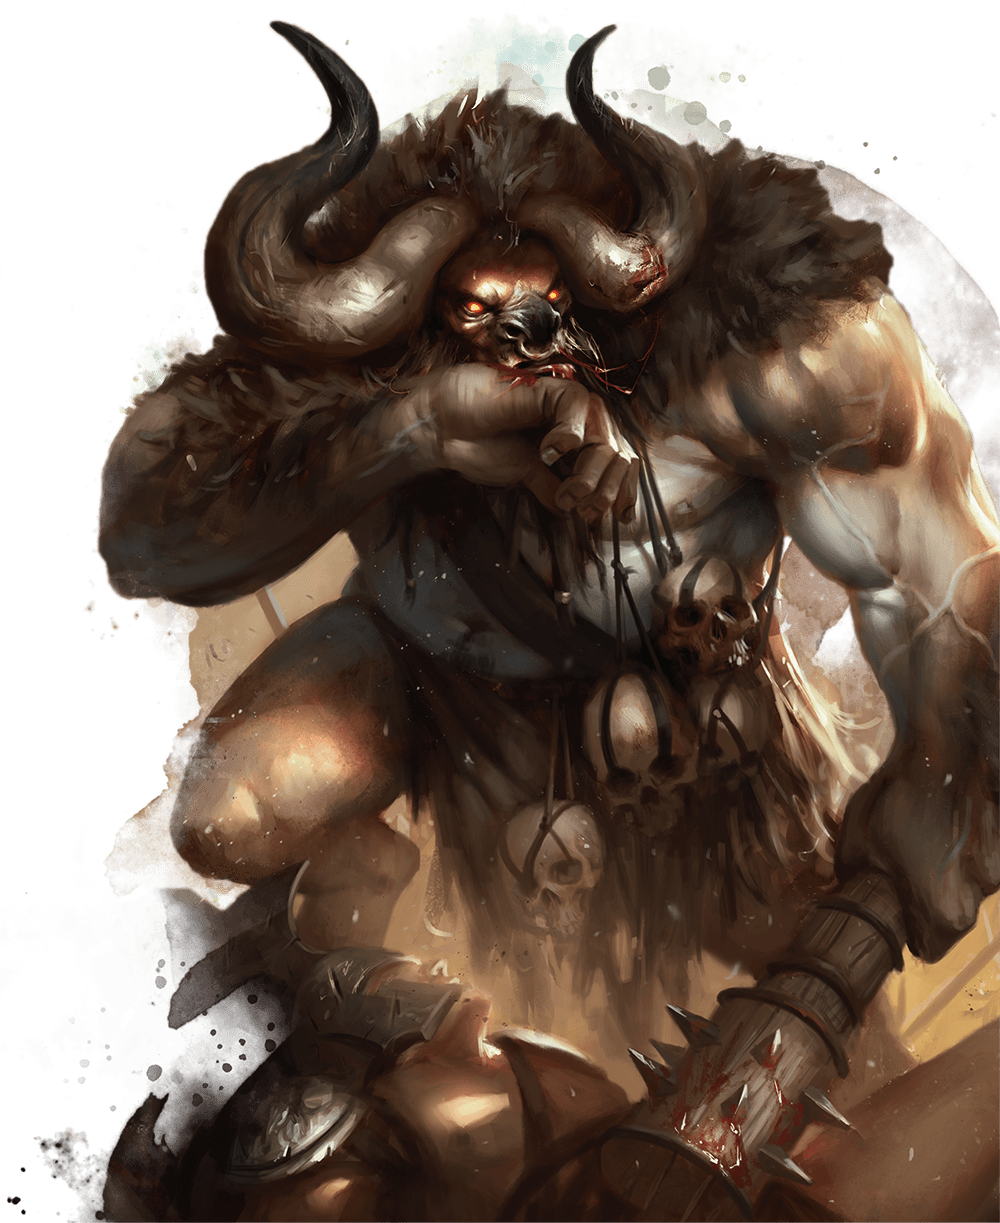
\includegraphics[width=0.50\pdfpagewidth]{05background/img/20treb_gat}};
% \end{tikzpicture}
%
% \newpage

\subsection*{Criminal} \label{ssec::criminal}
    Bandits, pirates, spies, and thieves all share a penchant for crime.
    You are an experienced criminal with a history of breaking the law.
    You have spent a lot of time among other criminals and still have contacts within the criminal underworld.
    You're far closer than most people to the world of murder, theft, and violence that pervades the underbelly of civilization, and you have survived up to this point by flouting the rules and regulations of society.

    There are many kinds of criminals, and within a thieves' guild or similar criminal organization, individual members have particular specialties.
    Even criminals who operate outside of such organizations have strong preferences for certain kinds of crimes over others.
    Choose the role you played in your criminal life.

    \subparagraph{Competences} Deception, plus your choice of two from among Intimidation, Sleight of Hand, Stealth, or a set of Thieves' Tools.

    \subparagraph{Equipment} A crowbar, a black cloak with a hood, a set of dark common clothes, and a knife.

    \subsubsection{Thieves' Cant}
        You know Thieves' cant, a secret mix of dialect, jargon, and code that allows you to hide messages in seemingly normal conversation.
        Only another creature that knows thieves' cant understands such messages.
        It takes four times longer to convey such a message that it does to speak the same idea plainly.

        In addition, you understand a set of secret signs and symbols used to convey short, simple messages, such as whether an area is dangerous or the territory of a thieves' guild, whether loot is nearby, or whether the people in an area are easy marks or will provide a safe house for thieves on the run.
    % ========================================================================== %

\subsection*{Entertainer} \label{ssec::entertainer}
    Acrobats, athletes, gladiators, and performers all share a passion for self-improvement, their art, and entertainment. % Considering athletes here is a bit shit but is the best I can do tbh.
    You thrive in front of an audience.
    You know how to entrance them, entertain them, and even inspire them.
    Whatever techniques you use, your art is your life.

    \subparagraph{Competences} Performance, plus your choice of two from among Acrobatics, Athletics, a musical instrument, or land vehicles.

    \subparagraph{Equipment} A tool related to your art (a musical instrument, a weapon, a leather ball, etc.), a lucky charm or past trophy, and costume clothes.

    \subsubsection{By Popular Demand} \label{feat::bypopulardemand}
        You can always find a place to perform, may it be an inn, a tavern, an arena, a field, or even in a noble's court.
        At such a place, you receive free lodging and food of a modest or comfortable standard (depending on the quality of the establishment), as long as you perform daily.
        In addition, your performance makes you something of a local figure.
        When strangers recognize you in a town where you have performed, they typically take a liking to you.
    % ========================================================================== %

\subsection*{Laborer} \label{ssec::laborer}
    Born a laborer, you have jumped through one odd job to the next through your entire life.
    One day you might be a farmhand, another a miner, then a servant, and later a stevedore.
    You adapt as is required, with a sharp nose for coin.

    You have dirt under your fingernails and never shy away from a little hard work.
    Most of your time is filled in back-breaking labor, the type of work that keeps merchants and mine owners in business.% even as it makes you just enough money to get by.
    It’s a hard life, but it’s toughened you and made you confident in your abilities.

    \subparagraph{Competences} Athletics, plus your choice of two from among Animal Handling, Survival, land vehicles, or a set of artisan's tools of your choice.

    \subparagraph{Equipment} A job-related tool (choose a piece of equipment that costs 2 agnomas or less), small knife, a set of bone dice or a deck of Huathem cards, and a set of common clothes.

    \subsubsection{Hired Hand}
        As one of the working class, finding work and a place to stay is easy for you.
        In any location that needs workers, you can find room and board for you and your companions.
        You also get enough money for a poor lifestyle for as long as the work holds out, unless you or your companions prove to be a danger to those around you.
        Your employer and the other laborers may even protect you from the law or anyone else searching for you, though they will not risk their lives for you.
    % ========================================================================== %

\subsection*{Merchant} \label{ssec::merchant}
    Caravan masters, shopkeepers, and traders all focus on one thing: coin.
    You don't craft items yourself but earn a living by buying and selling the works of others (or the raw materials artisans need to practice their craft).
    You might be part of a large merchant consortium or family with interests across the region. Perhaps you transported goods from one place to another, by ship, wagon, or caravan, or bought them from traveling traders and sold them in your own little shop.

    \subparagraph{Competences} Persuasion, plus your choice of two from among Investigation, a set of navigator's tools, one language, or land vehicles.

    \subparagraph{Equipment} A mule and cart, a merchant's scale, a set of fine clothes, and a belt containing 10 agnomas (nickel coins, see page \pageref{sec::currency}).

    \subsubsection{Supply Chain} \label{feat::supplychain}
        From your time as a merchant, you retain connections with wholesalers, suppliers, and other merchants and entrepreneurs.
        You can call upon these connections when looking for items or information.
        In locations where you are not familiar, you are able to establish this web of connections as part of a long rest.
    % ========================================================================== %

\subsection*{Noble} \label{ssec::noble}
    You understand wealth, power, and privilege.
    You carry a noble title, and your family owns land, collects taxes, and wields significant political influence.
    You might be a pampered aristocrat unfamiliar with work or discomfort, a former merchant just elevated to the nobility, or a champion who gained status via knighthood.
    Or you could be an honest, hard-working landowner who cares deeply about the people who live and work on your land, keenly aware of your responsibility to them.

    \subparagraph{Competences} History, plus your choice of two from among Deception, Persuasion, Religion, or a language of your choice.

    \subparagraph{Equipment} A set of fine clothes, and signet ring with your family's sigil, and a purse containing 25 agnomas.

    \subsubsection{Position of Priviledge}
        Thanks to your noble birth, people are inclined to think the best of you.
        You are welcome in high society, and people assume you have the right to be wherever you are.
        The common folk make every effort to accommodate you and avoid your displeasure, and other people of high birth treat you as a member of the same social sphere.
        You can secure an audience with a local noble if you need to.

        % \thispagestyle{empty}
        % \begin{tikzpicture}[remember picture,overlay]
        %     \node[anchor=south west, xshift=-0.10cm, yshift=-0.10cm] at (current page.south west) {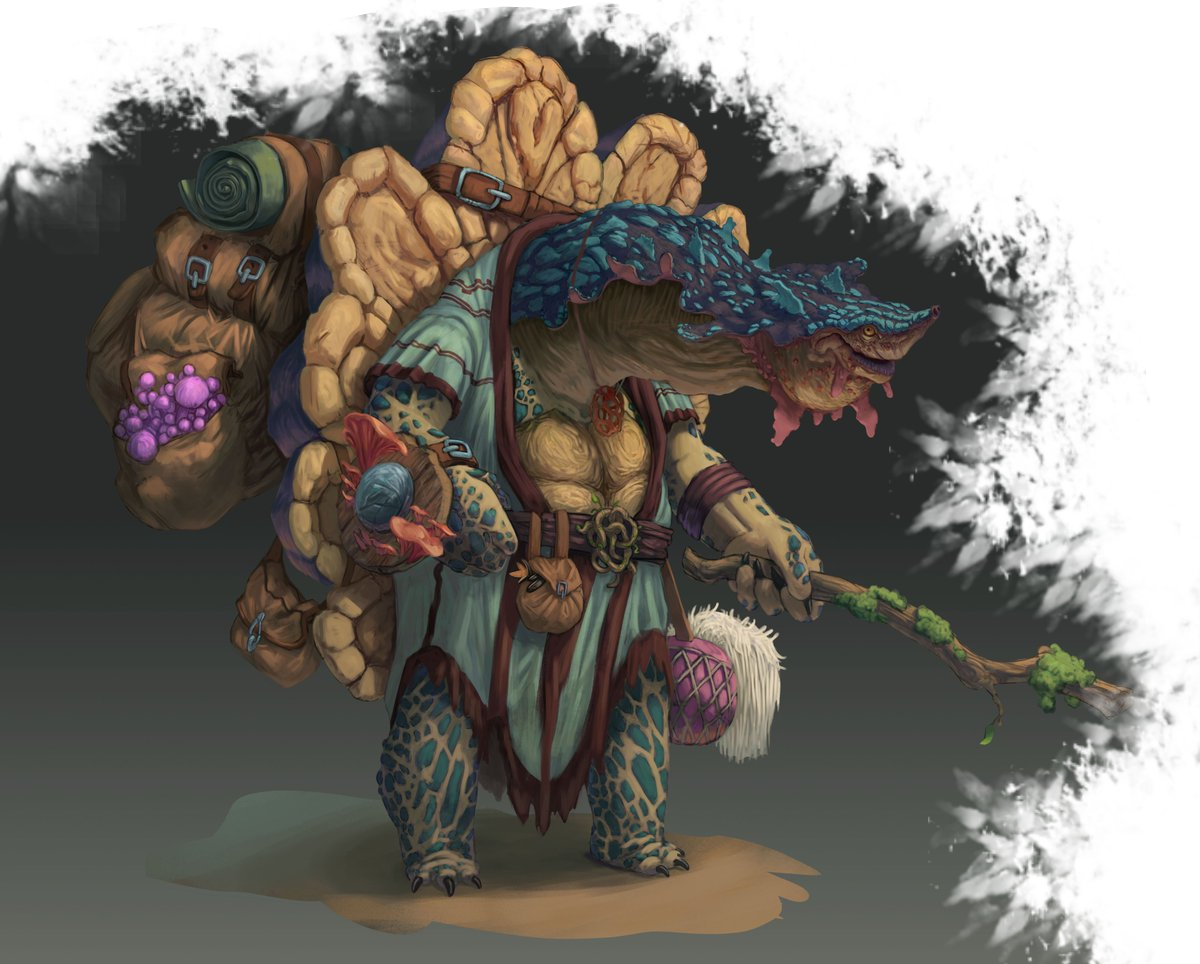
\includegraphics[width=0.52\pdfpagewidth]{05background/img/20tortle_mycolomancer}};
        % \end{tikzpicture}
        %
        % \newpage

        You can exert leverage over one or more individuals below you in the social hierarchy and demand their help as needs warrant.
        For example, you can have a message carried across a neighborhood, procure a short carriage ride without paying, or have others clean up a bloody mess you left in an alley.
        The DM decides if your demands are reasonable and if there are people available and willing to fulfill them.
        As your social status improves, you gain influence over more people, including ones in greater positions of power.
    % ========================================================================== %

\subsection*{Sailor} \label{ssec::sailor}
    You sailed on a seagoing vessel for years.
    In that time, you faced down mighty storms, monsters of the deep, and those who wanted to sink your craft to the bottomless depths.
    Your first love is the distant line of the horizon.

    Discuss the nature of the ship you previously sailed with your Dungeon Master.
    Was it a merchant ship, a naval vessel, a ship of discovery, or a pirate ship?
    How famous (or infamous) is it?
    Is it widely traveled?
    Is it still sailing, or is it missing and presumed lost with all hands?
    What were your duties on board?

    \subparagraph{Competences} Water vehicles, plus your choice of two from among Perception, Survival, Navigator's Tools, or Carpenter's Tools.

    \subparagraph{Equipment} A belaying pin, 50 feet of silk rope, a lucky charm, and a set of common clothes.

    \subsubsection{Ship's Passage}
        When you need to, you can secure free passage on a sailing ship for yourself and your companions.
        You might sail on the ship you served on, or another ship you have good relations with (perhaps one captained by a former crewmate).
        Because you're calling in a favor, you can't be certain of a schedule or route that will meet your every need.
        Your Dungeon Master will determine how long it takes to get where you need to go.
        In return for your free passage, you and your companions are expected to assist the crew during the voyage.
    % ========================================================================== %

\subsection*{Scholar} \label{ssec::scholar}
    Sages, scholars, students, and scientists are all passionate about one or many fields of study.
    You are defined by your extensive studies, and your characteristics reflect this life of study.
    Devoted to scholarly pursuits, you value knowledge highly --- sometimes in its own right, sometimes as a means toward other ideals.

    \subparagraph{Competences} Investigation, plus your choice of two from among Arcana, History, Medicine, or one language.

    \subparagraph{Equipment} A bottle of black ink, a quill, a small knife, a letter from a dead colleague posing a question you have not yet been able to answer, and a set of common clothes.

    \subsubsection{Researcher} \label{feat::researcher}
        When you attempt to learn or recall a piece of lore, if you do not know that information, you often know where and from whom you can obtain it.
        Usually, this information comes from a library, scriptorium, university, or a sage or other learned person or creature.
        Your DM might rule that the knowledge you seek is secreted away in an almost inaccessible place, or that it simply cannot be found.
    % ========================================================================== %

\subsection*{Soldier} \label{ssec::soldier}
    You trained as a youth, studied the use of weapons and armor, learned basic survival techniques. %, including how to stay alive on the battlefield.
    You might have been part of a standing army or a mercenary company, or perhaps a member of a local militia who rose to prominence during a recent war.

    % \newpage

    When you choose this background, work with your DM to determine which organization you were a part of, how far through its ranks you progressed, and what kind of experiences you had during your career.
    Was it a standing army, a town guard, or a village militia?
    Or it might have been a noble's order of knights, a merchant's private army, or a mercenary company.

    \subparagraph{Competences} Competence with a weapon type of your choice, plus your choice of two from among Athletics, Intimidation, an armor type of your choice, or land vehicles.

    \subparagraph{Equipment} An insignia of rank, a trophy taken from a fallen enemy, and a set of common clothes.

    \subsubsection{Military Rank}
        You have a military rank from your career as a soldier.
        Soldiers loyal to your former military organization still recognize your authority and influence, and they defer to you if they are of a lower rank.
        You can invoke your rank to exert influence over other soldiers and requisition simple equipment or horses for temporary use.
        You can also usually gain access to friendly military encampments and fortresses where your rank is recognized.
    % ========================================================================== %

\subsection*{Outlander} \label{ssec::outlander}
    Either by choice or by birthright, you have spent much of your life in the wilds, far from the comforts of civilization.
    You've witnessed the migration of herds larger than forests, survived weather more extreme than any city-dweller could comprehend, and enjoyed the solitude of being the only thinking creature for miles in any direction.
    The wilds are in your blood, whether you were a nomad, an explorer, a recluse, a hunter-gatherer, or a hermit.
    Even in places where you don't know the specific features of the terrain, you know the ways of the wild.

    \subparagraph{Competences} Survival, plus your choice of two from among Animal Handling, Athletics, Nature, or a musical instrument.

    \subparagraph{Equipment} A staff, a hunting trap, a trophy from nature, and a set of traveler's clothes.

    \subsubsection{Wanderer}
        % You have an excellent memory for maps and geography, and you can always recall the general layout of terrain, settlements, and other features around you.
        You can always recall the general layout of terrain, settlements, and other features around you.
        In addition, you can find food and fresh water for yourself and up to five other people each day, provided that the land offers berries, small game, water, and so forth.
    % ========================================================================== %

\newpage

% Strength
%     !3 Athletics
% Dexterity
%     .1 Acrobatics
%     .2 Sleight of Hand
%     .1 Stealth
% Intelligence
%     .1 Arcana
%     !2 History
%     !1 Investigation
%     .1 Nature
%     !1 Religion
% Wisdom
%     .2 Animal Handling
%     .2 Insight
%     .1 Medicine
%     .2 Perception
%     !2 Survival
% Charisma
%     !1 Deception
%     .2 Intimidation
%     !1 Performance
%     !2 Persuasion
% !0 Weapon
% .1 Armor
% !6 Tools
% .2 Instrument
% .4 Languages
% .4 Vehicles (land)
% !0 Vehicles (water)
% .0 Vehicles (air)
